\documentclass[pointlessnumbers,DIV12,a5paper,twoside,bibtotocnumbered]{scrartcl}

%       $Id: latex-tutorium.tex,v 1.30 2005/06/28 14:20:34 bronger Exp $    
%
%     latex-tutorium.tex -- Part of the LaTeX Tutorium
%     Copyright 2004 Torsten Bronger <bronger@users.sourceforge.net>,
%                    
%
%   This program is free software; you can redistribute it and/or
%   modify it under the terms of the Artistic License 2.0 as published
%   by Larry Wall.  You should have received a copy of the Artistic
%   License 2.0 along with this program in the file COPYING; if not,
%   you can get it at
%     http://dev.perl.org/rfc/346.html
%   or contact the current maintainers of the LaTeX Tutorium.
%
%   This program is distributed in the hope that it will be useful, but
%   WITHOUT ANY WARRANTY; without even the implied warranty of
%   MERCHANTABILITY or FITNESS FOR A PARTICULAR PURPOSE.  See the
%   Artistic License 2.0 for more details.
%
%   This file may only be distributed together with a copy of the LaTeX
%   Turorium.
%
%   The LaTeX Tutorium consists of all files listed in manifest.txt.

\usepackage[nofoot,a5paper,
lmargin=1.9cm,rmargin=2.1cm,
tmargin=1.2cm,bmargin=2.3cm,
headheight=0.52cm,
headsep=0.5cm,includehead]{geometry}[2002/07/08]

\usepackage{scrpage2}
\pagestyle{scrheadings}
\clearscrheadfoot
\makeatletter
\@tempdima\textwidth
\advance\@tempdima0.8cm
\setheadwidth[0pt]{\@tempdima}
\makeatother
\cehead{\rightmark}
\cohead{\leftmark}
\rohead{\relax\hbox to 0.8cm{\hfill\pagemark}}
\lehead{\hbox to 0.8cm{\pagemark\hfill}\relax}
\automark[section]{section}
\setheadsepline{0.4pt}

\usepackage[latin1]{inputenc}
\usepackage[T1]{fontenc}
\usepackage{graphicx,mathptmx,courier,textcomp,booktabs,relsize,wrapfig,
  keystroke,fixltx2e}
\usepackage[scaled]{helvet}

\usepackage{ngerman}
\usepackage[sort&compress,numbers]{natbib}

\newif\ifminion
\IfFileExists{minioneu.sty}{\miniontrue}{\minionfalse}
\ifminion
  \usepackage{germhyph}
  \usepackage{minioneu}
  \usepackage{soul}
  \capsselect{narrow}
  \newcommand*{\versalien}[1]{{\smaller\hskip0pt\caps{#1}}}
  \newcommand*{\textebf}[1]{{\fontseries{eb}\selectfont #1}}
  \else
  \newcommand*{\versalien}[1]{{\smaller#1}}
  \newcommand*{\textebf}[1]{\textbf{#1}}
  \fi

\makeatletter
\DeclareRobustCommand{\LaTeX}{L\kern-.26em%
        {\sbox\z@ T%
         \vbox to\ht\z@{\hbox{\check@mathfonts
                              \fontsize\sf@size\z@
                              \math@fontsfalse\selectfont
                              A}%
                        \vss}%
        }%
        \kern-.15em%
        \TeX}
\makeatother

\renewcommand{\topfraction}{.9}
\renewcommand{\bottomfraction}{.9}
\renewcommand{\textfraction}{.1}
\renewcommand{\dbltopfraction}{.9}

\usepackage[german]{varioref}
\usepackage{amsmath}
\DeclareMathOperator{\Rect}{rect}

\usepackage{listings,color}
\lstset{language=[LaTeX]TeX,columns=[l]fullflexible,
  basicstyle=\ttfamily,extendedchars=true,
  numberstyle=\sffamily\scriptsize,keepspaces,keywords={includegraphics,toprule,
    midrule,bottomrule,maketitle,tableofcontents,intertext,notag,
    url}}%,backgroundcolor=\color[gray]{0.9}}

\newcommand{\WYSIWYG}{\versalien{WYSIWYG}}
\newcommand{\PDF}{\versalien{PDF}}
\newcommand{\PNG}{\versalien{PNG}}
\newcommand{\GIF}{\versalien{GIF}}
\newcommand{\TIFF}{\versalien{TIFF}}
\newcommand{\BMP}{\versalien{BMP}}
\newcommand{\EPS}{\versalien{EPS}}
\newcommand{\CD}{\versalien{CD}}
\newcommand{\JPEG}{\versalien{JPEG}}

\newcommand{\TeXnicCenter}{\TeX\-nic\-Cen\-ter}

\newcommand*{\NZB}[1]{\marginline{\scriptsize\raggedright\hspace{0pt}#1\par}}

\newcommand{\Package}[1]{\texttt{#1}}
\newcommand{\Environment}[1]{\texttt{#1}}
\newcommand{\Parameter}[1]{\textrm{\itshape <#1>}}
\title{\vspace*{-2cm}Das \LaTeX-Tutorium}

\author{Torsten Bronger\thanks{bronger@physik.rwth-aachen.de} \and Christian
  Faulhammer \and Mark Trettin}

\date{\today\vspace*{-1.3cm}}
\sloppy

\usepackage{url,fancybox,pifont}
\urlstyle{sf}

% \usepackage[activate]{pdfcprot}

\ifpdfoutput{%
  \usepackage{hyperref}
  \hypersetup{%
    pdfauthor={Torsten Bronger,Christian Faulhammer,Mark Trettin},%
    pdftitle={Das LaTeX-Tutorium},%
    pdfsubject={Einf�hrung in LaTeX f�r Windows},%
    pdfkeywords={LaTeX,Tutorium,Tutorial,TeXnicCenter,Einf�hrung}
  }
}%

\hyphenation{Text-ein-ga-be Zei-len-um-bruch Texte Home-page}

\newdimen{\Hinweisbreite}
\newenvironment{Hinweis}[1][\ding{46}]{\removelastskip\bigskip\noindent\fboxsep0.4cm
  \Hinweisbreite\hsize\advance\Hinweisbreite-2\fboxsep\advance\Hinweisbreite-2\fboxrule
  \shadowbox\bgroup\begin{minipage}{\Hinweisbreite}%
    \hangindent=1cm\hangafter=-2\parindent0pt\parskip1.5ex
    \leavevmode\hbox to 0pt{\hss\Huge\vtop to
      0pt{\vskip-0.5ex\hbox to 0.9cm{\hfill#1\hfill}\vss}\hskip0.1cm}\ignorespaces}
  {\par\end{minipage}\egroup\bigskip}

\begin{document}

% Allgemeine Richtlinien:
%
% Der Plan ist, von der alten Methode, LaTeX zu erl�utern, wegzukommen.  Der
% ganze historische Ballast wird sofort aufgegeben.  Das hei�t z.B.:
%
%               Ja                                            Nein
% --------------------------------------------------------------------------------------
%  Editor in den Vordergund stellen     Das (La)TeX-Programm in den Vordergrund stellen
%  Heutige "best common practice"       Darstellung veralteter Methoden und Pakete
%  Allgemein bekannte Layout-Elemente   Feinheiten der Typographie, z.B. Ligaturen
%  Plakative Darstellung                Hintergrundwissen
%  Konzentration auf Windows            Besprechung aller Plattformen
%  Klare Software-Liste                 Software-Liste mit etlichen Alternativen
%  PDF                                  DVI/PS
%  Times & Co.                          Computer Modern
%  KOMA-Script                          Standard-Klassen
%  inputenc, T1                         "u etc., OT1
%  Babel                                german.sty
%  Syntax-Highlighting                  Einfache Schreibmaschinenschrift
%
%
% Die Hoffnung ist, dadurch einen maximal effektiven Einstieg zu erm�glichen.
% Es ist eine \emph{Einf�hrung} ("Tutorial") und kein Lehrbuch, das dem Anspruch
% der Umfassendheit gen�gen will.
%
% Es soll aber ein in sich geschlossenes B�chlein darstellen.  Die typischen
% Elemente eines Dokuments sollen abgedeckt werden.

% Wenn man die folgende Zeile einkommentiert, wird eine ``Nullte'' Seite
% ausgespuckt.  Der Grund daf�r ist, da� man dann ein Postscript erzeugen kann
% und mit
%
% pstops "2:0L(21cm,0cm)+1L(21cm,14.85cm)" latex-tutorium.ps out.ps
%
% eine A4-Version mit zwei (sich gegen�berliegenden!) Seiten auf einem Blatt
% erh�lt.  Ich will aber nicht ausschlie�en, da� das auch einfacher geht.
%
%\thispagestyle{empty}~\clearpage\setcounter{page}{1}

% Eine mit Blattschneider auf echtes A5 trimmbare Version bekommt man, wenn man
% nichts weiter einkommentiert, ein Postscript erzeugt (Vorsicht! Wegen
% mangelnder PNG-Unterst�tzung und fehlendem CP suboptimale Qualit�t!) und dann
%
% pstops "4:0L(21cm,0cm)+2L(21cm,14.85cm),3L(21cm,0cm)+1L(21cm,14.85cm)" \
%     latex-tutorium.ps out.ps
%
% aufruft.

\maketitle
\tableofcontents
\cleardoublepage
%       $Id: einfuehrung.tex,v 1.15 2005/06/28 14:20:25 bronger Exp $    
%
%     einfuehrung.tex -- Part of the LaTeX Tutorium
%     Copyright 2004 Project Members of
%                    http://sourceforge.net/projects/latex-tutorium/
%                    
%
%   This program is free software; you can redistribute it and/or
%   modify it under the terms of the Artistic License 2.0 as published
%   by Larry Wall.  You should have received a copy of the Artistic
%   License 2.0 along with this program in the file COPYING; if not,
%   you can get it at
%     http://dev.perl.org/rfc/346.html
%   or contact the current maintainers of the LaTeX Tutorium.
%
%   This program is distributed in the hope that it will be useful, but
%   WITHOUT ANY WARRANTY; without even the implied warranty of
%   MERCHANTABILITY or FITNESS FOR A PARTICULAR PURPOSE.  See the
%   Artistic License 2.0 for more details.
%
%   This file may only be distributed together with a copy of the LaTeX
%   Turorium.
%
%   The LaTeX Tutorium consists of all files listed in manifest.txt.

\section{Was ist \LaTeX?}

\LaTeX{} ist ein Computer-Programm, mit dem man Texte schreiben kann.  Seien es
kurze Memos, Briefe, l�ngere Berichte, Studienarbeiten oder auch ganze B�cher:
\LaTeX{} kommt mit allen wichtigen Textsorten problemlos zurecht.  F�r jeden
dieser F�lle garantiert \LaTeX{} ein professionelles, perfekt gestaltetes
Layout.

\LaTeX{} legt dabei besonderen Wert auf drei Dinge:
\begin{enumerate}
\item Bei der Eingabe des Textes soll sich der Autor voll auf seinen Text
  konzentrieren k�nnen, und nicht von �u�erlichkeiten abgelenkt werden.
\item Beim Ausdruck des Textes wird bestm�gliche Qualit�t abgeliefert, selbst
  wenn der Autor von solchen Dingen keine oder kaum Ahnung hat.  Es wird dabei
  ein Niveau erreicht, das beispielsweise mit Word nicht zu realisieren ist.
\item Zuverl�ssigkeit.  Der Kern von \LaTeX{} gilt als einer der stabilsten und
  fehler-freiesten �berhaupt.  Selbst bei sehr komplexen Dokumenten, z.\,B. mit
  vielen Grafiken und Tabellen, bleibt das Programm belastbar und schnell.
\end{enumerate}

\noindent
\LaTeX{} ist kostenlos.  Es wurde von tausenden von Software-Entwicklern,
Ingenieuren, Forschern, Studenten und Enthusiasten auf der ganzen Welt
programmiert und der Allgemeinheit zur Verf�gung gestellt.  Au�erdem verbessern
und erweitern diese Leute \LaTeX{} st�ndig.  Es wird viel an der Hochschule
eingesetzt, aber auch in Verlagen f�r B�cher und wissenschaftliche
Zeitschriften.  Der Kern von \LaTeX{} kommt t�glich hunderttausendfach bei der
Deutschen Bahn und der Telekom zum Einsatz.

\medskip
Soweit es das Erzeugen von Dokumenten angeht, ist \LaTeX{} ein vollwertiger
Ersatz f�r Textverarbeitungsprogramme wie Word.  Es ist alles dabei, was das
Herz begehrt: Formatierung, Schriftarten, Grafiken, Tabellen, Aufz�hlungen,
Fu�noten, Querverweise, Rechtschreibkontrolle, automatische Verzeichnisse, etc.

Es gibt sogar einige Dinge, die \LaTeX{} den meisten anderen Programmen voraus
hat.  Drei Beispiele:
\begin{itemize}
\item \LaTeX{} kann selbstst�ndig f�r alle Abbildungen und Tabellen des Dokumentes
  die bestm�glichen Pl�tze suchen.  Obwohl der Autor das auch �berstimmen kann,
  lernt man diese Hilfe schnell zu sch�tzen.
\item Leute, die ihren Dokumenten Literaturverzeichnisse anf�gen m�ssen, k�nnen
  das zu einem guten St�ck automatisch durch \LaTeX{} erledigen lassen.
\item \LaTeX{} verf�gt �ber den wohl besten Formelsatz der Welt.  Das n�tzt
  beileibe nicht nur Mathematikern; formelartige Ausdr�cke kommen in den
  meisten technischen und wissenschaftlichen Dokumenten, und selbst in den
  Sprach"~, Gesellschafts- und Geisteswissenschaften vor.
\end{itemize}
\nopagebreak
Dieses Tutorium ist nat�rlich auch mit \LaTeX{} gemacht worden.

\subsection*{Kein \WYSIWYG}
\index{WYSIWYG@\WYSIWYG}

\LaTeX{} hat allerdings eine gew�hnungsbed�ftige Eigenart:

In Word tippt man seinen Text, und man sieht ihn dabei auf dem Bildschirm so,
wie er sp�ter aus dem Drucker kommt.  Man nennt diese Technik "`\WYSIWYG"'\@.
Es ist eine komfortable M�glichkeit der Texteingabe.

\LaTeX{} geht einen anderen Weg.  Man tippt seinen Text, sieht dabei jedoch nur
den Text selber, ohne Formatierung.  Stattdessen steuert man die Formatierung
in Form von ausgeschriebenen Befehlen im Text.  Das ist am Anfang ziemlich
un�bersichtlich, aber man gew�hnt sich rasch daran.  Keine Sorge: Es gen�gt ein
Tastendruck, um jederzeit am Bildschirm das Endergebnis zu sehen, und zwar noch
akkurater als mit Word.

Das ist quasi eine Not, aus der \LaTeX{} eine Tugend macht.  Zum einen ist der
Verzicht auf \WYSIWYG{} ein wichtiger Grund f�r die Zuverl�ssigkeit von
\LaTeX{}, \WYSIWYG{} ist n�mlich eine sehr aufw�ndige und daher etwas
anf�llige Technik.

Zum anderen hat man seine Ruhe vor Layout-Fragen.  Wenn man will, kann man zwar
auch mit \LaTeX{} das Layout nahezu beliebig beeinflussen, was aber nicht immer
empfehlenswert ist: Die Vorgaben der Profis, die \LaTeX{} gemacht haben, sorgen
schon f�r ein hervorragendes Resultat.

Man muss �brigens kein Englisch sprechen, um \LaTeX{} zu bedienen; es hilft
allerdings dabei, sich die Befehle zu merken.


\subsection*{�ber dieses Turorium}

Dieser Text ist eine sehr konkrete Einf�hrung in \LaTeX\@.  Mit "`konkret"' ist
gemeint, dass dieser Text den Anspruch hat, einen Neuling ganz von Anfang an
bis zum erfolgreichen Benutzen von \LaTeX\ zu begleiten.  Das schlie�t
insbesondere das Herankommen an \LaTeX, die Installation, und die Bedienung des
Editors ein.  Dieses Tutorium richtet sich an Windows-Benutzer.

Es handelt sich hier aber nicht um eine vollst�ndige \LaTeX"=Beschreibung.
Daf�r sind andere zust�ndig (siehe die Literatur-Liste auf
Seite~\pageref{sec:literatur}.)

Die Autoren sind Mitglieder der Aachener \TeX-Gruppe.  Der Text darf frei
verteilt und ausgedruckt werden.  Siehe `\url{latex-tutorium.sourceforge.net}'.

%%% Local Variables: 
%%% mode: latex
%%% TeX-master: "latex-tutorium"
%%% End: 


%       $Id: installation.tex,v 1.17 2005/06/28 18:30:35 bronger Exp $    
%
%     installation.tex -- Part of the LaTeX Tutorium
%     Copyright 2004 Project Members of
%                    https://github.com/latextemplates/latex-tutorium/
%                    
%
%   This program is free software; you can redistribute it and/or
%   modify it under the terms of the Artistic License 2.0 as published
%   by Larry Wall.  You should have received a copy of the Artistic
%   License 2.0 along with this program in the file COPYING; if not,
%   you can get it at
%     http://dev.perl.org/rfc/346.html
%   or contact the current maintainers of the LaTeX Tutorium.
%
%   This program is distributed in the hope that it will be useful, but
%   WITHOUT ANY WARRANTY; without even the implied warranty of
%   MERCHANTABILITY or FITNESS FOR A PARTICULAR PURPOSE.  See the
%   Artistic License 2.0 for more details.
%
%   This file may only be distributed together with a copy of the LaTeX
%   Turorium.
%
%   The LaTeX Tutorium consists of all files listed in manifest.txt.


\section{Die Installation unter Windows}
\index{Installation}
\index{Download}
\index{CD@\CD}

Es gibt mehrere M�glichkeiten, an \LaTeX{} heranzukommen:
\begin{itemize}
\item Man nutzt eine sehr gute Internet-Verbindung, um es sich herunterzuladen.
  Modem kann man vergessen, mit \versalien{ISDN} ist etwas Geduld n�tig.  Ab
  \versalien{DSL} aufw�rts geht es mehr oder minder flott.
\item Man kauft sich eine \versalien{CD}\@.  Die gibt es f�r wenig Geld in
  einigen B�chereien (z.\,B. Lehmanns), man kann sie aber auch online
  bestellen.  Auf der \versalien{CD} ist u.\,U. nicht exakt das drauf, was hier
  im Tutorium verwendet wird.
\item Man kennt einen netten Menschen, der's hat.
\end{itemize}

\bigskip
\noindent
Von den folgenden vier Programmen m�ssen drei installiert sein, um mit \LaTeX{}
arbeiten zu k�nnen.  FreePDF ist nicht unbedingt n�tig.


\begin{table}
  \caption{Die Komponenten von \LaTeX{} zum Herunterladen.  Sie sollten in
      genau dieser Reihenfolge installiert werden.}
  \label{tab:Downloads}
  \vspace{1ex}
  \begin{tabular}{@{}llc@{}}
    \toprule
    Komponente       &  Homepage                 &  Gr��e          \\
                     &                           &  (Megabytes)    \\
    \midrule
    Acrobat Reader   &  \url{www.adobe.de}       &  $18$           \\
    MiK\TeX{}        &  \url{www.miktex.org}     &  $24$           \\
    FreePDF (optional)
                     &  \url{freepdfxp.de/fpxp.htm}&  $11$         \\
    \TeXnicCenter{}  &  \url{www.toolscenter.org}  &  $4$          \\
    \bottomrule
  \end{tabular}
\end{table}

\subsection{Acrobat Reader}
\index{Reader, Acrobat Reader}
\index{Acrobat Reader}
\index{Adobe}
\index{PDF@\PDF}

Mit ein bisschen Gl�ck ist der Acrobat Reader bereits auf dem Computer
vorhanden, weil es bei einigen anderen Programmen dabei ist.  Wenn nicht, muss
man es sich bei `\url{www.adobe.de}' herunterladen, das sind knapp 18\,MB\@.

Die Datei, die man dabei erh�lt, ruft man auf, und das ergibt dann alles
weitere.  Die Installation selber dauert nur zwei Minuten.


\subsection{\LaTeX}
\index{MiKTeX@MiK\TeX}

Nat�rlich braucht man \LaTeX{} selber.  Das bekommt man unter
`\url{www.miktex.org}' in Form vom sogenannten "`MiK\TeX"'.  Man kann es
entweder herunterladen (es sind allerdings mindestens 24~Megabytes) oder man
bestellt sich dort "`MiK\TeX{} on \versalien{CD-R}"'\@.

In beiden F�llen muss man das Setup-Programm aufrufen.  Wenn man von \CD{}
installiert, sollte man mindestens die "`Large"'-Installation w�hlen, ansonsten
reicht die "`Small"'-Variante.  Das ganze dauert je nach Fall zwischen f�nf und
f�nfzehn Minuten.


\subsection{FreePDF}
\label{sec:FreePDF}
\index{FreePDF}
\index{PDF}
\index{Ghostscript}
\index{Postscript}

Das Programm FreePDF ist nicht unbedingt f�r ein funktionierendes \LaTeX-System
n�tig.  Es erlaubt, aus jeder beliebigen Windows-Anwendung heraus \PDF-Dateien
zu erzeugen, die man als Bilder in \LaTeX{}-Texte einbinden kann.  Wir
empfehlen, es immer zu installieren, wenn man Abbildungen aus beispielsweise
Corel Draw, PowerPoint, Excel oder Origin in seinen Texten verwenden m�chte.

Es ist kostenlos im Internet unter `\url{freepdfxp.de/fpxp.htm}' zu beziehen.
Dort klickt man auf "`Download"' und mu� \emph{zwei} Dateien herunterladen und
installieren:
\begin{enumerate}
\item "`GhostScript"' ($10$~MByte) und
\item "`FreePDF~XP"' selber ($0{,}5$~MByte).
\end{enumerate}


\subsection{Der Editor}
\index{Editor}
\index{TeXnicCenter@\TeXnicCenter}
\index{ToolsCenter}

F�r den Benutzer ist der wichtigste Teil von \LaTeX{} der \emph{Editor}.  Im
Editor gibt man seinen Text ein, schaut ihn sich in der Schnellvorschau an und
druckt ihn aus.  In diesem Tutorium verwenden wir einen Editor namens
\TeXnicCenter.  Es gibt Alternativen, aber der \TeXnicCenter{} ist leicht zu
handhaben und bietet alles, was man braucht.  Seine Webseite ist
`\url{www.toolscenter.org}'.

Man bekommt ihn direkt aus dem Internet unter
\begin{quote}
  \url{http://www.texniccenter.org/front_content.php?idcat=50}
\end{quote}
Man muss dort die oberste Datei ausw�hlen (auf "`SourceForge.net"' klicken,
$5{,}5$\,MByte) und auf dem eigenen Rechner starten.  W�hrend der Installation
best�tigt man alle Vorgaben.  \textebf{Achtung:} Der \TeXnicCenter{} sollte
stets als allerletztes installiert werden!


%%% Local Variables: 
%%% mode: latex
%%% TeX-master: "latex-tutorium"
%%% End: 


%       $Id: erstes-dokument.tex,v 1.25 2005/06/28 14:20:33 bronger Exp $    
%
%     erstes-dokument.tex -- Part of the LaTeX Tutorium
%     Copyright 2004 Project Members of
%                    http://sourceforge.net/projects/latex-tutorium/
%                    
%
%   This program is free software; you can redistribute it and/or
%   modify it under the terms of the Artistic License 2.0 as published
%   by Larry Wall.  You should have received a copy of the Artistic
%   License 2.0 along with this program in the file COPYING; if not,
%   you can get it at
%     http://dev.perl.org/rfc/346.html
%   or contact the current maintainers of the LaTeX Tutorium.
%
%   This program is distributed in the hope that it will be useful, but
%   WITHOUT ANY WARRANTY; without even the implied warranty of
%   MERCHANTABILITY or FITNESS FOR A PARTICULAR PURPOSE.  See the
%   Artistic License 2.0 for more details.
%
%   This file may only be distributed together with a copy of the LaTeX
%   Turorium.
%
%   The LaTeX Tutorium consists of all files listed in manifest.txt.

\section{Das erste Dokument}
\subsection{Erste Schritte}
\label{sec:ersteschritte}

\TeXnicCenter{} bietet im Gro�en und Ganzen die gewohnte Oberfl�che und
Men�struktur, die man unter Windows gewohnt ist. Das hei�t, man kann Dateien
speichern, �ffnen, den Quelltext ausdrucken und vieles mehr.

Fangen wir mal mit einem sehr einfachen \LaTeX-Dokument an.  Man startet also
den \TeXnicCenter{} und gibt Folgendes ein:
\begin{lstlisting}
\documentclass{scrartcl}

\begin{document}
Dies ist mein erster Text.
\end{document}
\end{lstlisting}
Dann speichert man das Dokument ab und dr�ckt \keystroke{Strg}+\keystroke{F7}
und~\mbox{\keystroke{F5}.}  Es �ffnet sich ein Fenster, in dem man den Text so
sehen kann, wie er auch sp�ter aus dem Drucker kommen wird.  In unserem Fall
ist das nur der Text "`Dies ist mein erster Text"'.

Aber was bedeutet das, was wir gerade getippt haben?  Die allererste Zeile
lautet
\begin{lstlisting}
\documentclass{scrartcl}
\end{lstlisting}
und gibt in den geschweiften Klammern die \emph{Klasse} bzw.\ \emph{Art} des
Dokumentes an.  Man hat die Wahl zwischen Buch (\mbox{scrbook}), Artikel
(\mbox{scrartcl}) und Brief (\mbox{scrlttr$2$}).  Die K�rzel sind aus
historischen Gr�nden zugegebenerma�en seltsam, aber das soll uns nicht st�ren.
"`Artikel"' und "`Buch"' sollte man nicht zu w�rtlich nehmen.  Die meisten
\LaTeX-Benutzer nehmen "`Buch"' f�r alles, was aus Kapiteln besteht, und
"`Artikel"' f�r den Rest.

\begin{Hinweis}
  In der ersten Zeile einer \LaTeX-Datei muss man sich f�r die \emph{Klasse}
  seines Textes entscheiden.  Soll es ein Buch werden, schreibt man
  \lstinline|\documentclass{scrbook}|, \mbox{ansonsten}
  \lstinline|\documentclass{scrartcl}|.
\end{Hinweis}

\lstinline{\documentclass} ist auch das erste Beispiel f�r etwas sehr wichtiges
in \LaTeX: den \LaTeX-Befehl.

\subsubsection{Die Anatomie eines \LaTeX-Befehls}
\label{sec:anatomie}

Wie schon erw�hnt, sieht man bei \LaTeX{} die Formatierung des Textes nicht
direkt wie in Word, sondern in Form von \emph{Befehlen}, die zwischen dem Text
stehen.  Der Editor f�rbt sie zur besseren �bersicht blau ein, und hier im
Turorium schreiben wir sie im Fettdruck.

Unser kleines \LaTeX-Beispiel begann ja mit
\begin{lstlisting}
\documentclass{scrartcl}
\end{lstlisting}
Das ist ein typischer \LaTeX-Befehl.  Wie schon gesagt, bedeutet er, dass wir
einen Text ohne Kapitel schreiben wollen.  Ein \LaTeX-Befehl hat immer den
folgenden Aufbau:
\begin{enumerate}
\item Er beginnt mit einem umgekehrten Schr�gstrich~"`\verb|\|"', einem
  sogenannten "`Backslash"'.
\item Dann folgt der englische Name des Befehls, z.\,B. "`documentclass"' f�r
  "`Die Klasse des Dokumentes"'.
\item Als letztes kommen zus�tzliche Angaben, die sogenannten \emph{Parameter}.
  Sie stehen jeweils in geschweiften Klammern \lstinline|{...}|.  Je nach
  Befehl k�nnen es keiner, einer, oder mehrere Parameter sein.
  
  Meistens ist es aber genau einer, wie bei unserem Beispiel-Befehl, n�mlich
  eben das K�rzel "`scrartcl"'.
\end{enumerate}


\bigskip
Gut, soviel erstmal zu Befehlen.  Kommen wir nochmal zur�ck auf den
Beispieltext:
\begin{lstlisting}
\documentclass{scrartcl}

\begin{document}
Dies ist mein erster Text.
\end{document}
\end{lstlisting}
Da sind anscheinend noch zwei andere Befehle, \lstinline{\begin} und
  \lstinline{\end}.  In Wahrheit sind \lstinline{\begin} und \lstinline{\end}
aber ganz besondere Befehle, die eine \emph{Umgebung} umschlie�en.  Umgebungen
sind das zweitwichtigste in \LaTeX:

\subsubsection{Umgebungen}

Umgebungen klammern einen Bereich des Textes ein.  Unser Beispiel-Dokument von
vorhin enth�lt genau eine Umgebung, und es ist sogar die wichtigste, die immer
genau einmal vorkommen muss:
\begin{lstlisting}
\begin{document}
 ...
\end{document}
\end{lstlisting}
Die \lstinline|document|-Umgebung enth�lt den ganzen Text des Dokuments.  Jede
Umgebung beginnt mit
\begin{lstlisting}[escapeinside=`']
\begin{`\Parameter{Umgebungsname}'}
\end{lstlisting}
und endet mit
\begin{lstlisting}[escapeinside=`']
\end{`\Parameter{Umgebungsname}'}
\end{lstlisting}

Alles, was zwischen diesen Befehlen steht, erh�lt dieselben Eigenschaften und
wird als ein logisch zusammenh�ngender Teil behandelt.  Beispielsweise gibt es
Umgebungen, die den Text kleiner oder zentriert drucken.  Wie wir sp�ter sehen
werden, sind auch Aufz�hlungen und Tabellen Beispiele f�r Umgebungen.

\begin{Hinweis}
  Die wichtigste Umgebung ist \lstinline|\begin{document}|.  Mit ihr beginnt
    der eigentliche Text, der mit \lstinline|\end{document}| endet.
\end{Hinweis}


\subsubsection{Pakete -- L�sungen f�r alle Probleme}
\label{sec:pakete}

\LaTeX{} ist modular aufgebaut.  Neben den \LaTeX-Grundfunktionen gibt es noch
die \emph{Pakete}.  Pakete stellen in der Regel Zusatzfunktionen f�r bestimmte
Aufgaben bereit.  Beispielsweise gibt es Pakete zum Schreiben eines
Lebenslaufs.  Daneben gibt es aber auch Pakete, die bei jeder
\LaTeX-Installation garantiert vorhanden sind, weil sie so wichtige Dinge wie
Grafikeinbindung oder Textsprache bereitstellen.

Wie kann man \LaTeX-Pakete in Anspruch nehmen?  Zuerst einmal muss man den
Paketnamen f�r die entsprechende Aufgabe kennen und dann mit
\begin{lstlisting}[escapeinside=`']
\usepackage[`\Parameter{Optionen}']{`\Parameter{Paketname}'}
\end{lstlisting}
einf�gen.  Die Optionen in eckigen Klammern sind nicht bei allen Paketen n�tig.

Wichtig ist, \emph{wo} man Pakete einf�gt.  Vielleicht kam schon eben die Frage
auf, warum diese \lstinline{document}-Umgebung n�tig ist, wenn doch ohnehin
scheinbar alles da hineinwandert.  Nun, nicht alles.  Alle Pakete m�ssen
\emph{vor} der \lstinline{document}-Umgebung eingebunden werden.

\begin{Hinweis}
  Der Bereich, in dem man die Pakete einbindet, befindet sich zwischen
  \lstinline|\documentclass{...}| und \lstinline|\begin{document}|.  Man nennt
    diesen Bereich den \emph{Vorspann} oder die \emph{Pr�ambel}.
\end{Hinweis}
  
Abschlie�end, bevor wir das erste kompliziertere Dokument eingeben, sei hier
noch einmal der Grundaufbau einer \LaTeX-Datei dargestellt:
\begin{lstlisting}[escapeinside=`']
\documentclass{`\Parameter{Dokumentklasse}'}

\usepackage{...}  `\hspace{3em}\textrm{\textit{Pr�ambel}}'
\usepackage{...}

\begin{document}
Hier der Text ...
\end{document}
\end{lstlisting}


\subsection{Die Muster-Datei}
\label{Minimaldokument}

Ein Mini-Beispiel haben wir nun hinter uns, aber wie im letzten Abschnitt schon
angedeutet, kommt man ohne Zusatzpakete nicht sehr weit.  Blo� welche Pakete
ben�tigt man f�r den Anfang, und wie sind sie einzubinden?  Um diese Aufgabe
sp�rbar zu vereinfachen, wird nun ein Muster-Dokument vorgestellt, das man als
Ausgangspunkt f�r alle eigenen Dokumente benutzen kann.

Im Wesentlichen geht es um eine Muster-\emph{Pr�ambel}.  Vorsicht: Die sieht
zun�chst einmal etwas erschreckend aus.  Das meiste kann man ruhig so
hinnehmen.  Nur wenn es n�tig ist, werden wir auf den folgenden Seiten auf die
ein oder andere Zeile besonders eingehen.

\begin{lstlisting}[numbers=left,basicstyle=\ttfamily\ifminion\else\footnotesize\fi,
  escapeinside=`']
\documentclass{scrartcl}       % keine Kapitel
\usepackage[ansinew]{inputenc}   `\label{lst:start-pakete}'
\usepackage[T1]{fontenc}
\usepackage{graphicx,textcomp,booktabs,amsmath}
\usepackage{mathptmx,courier}    `\label{lst:mathptmx-courier}'
\usepackage[scaled]{helvet}      `\label{lst:helvet}'

\usepackage[ngerman]{babel}    % Neue Rechtschreibung `\label{lst:ngerman}'

\begin{document}               % Hier geht der Text los

Hallo! Dies ist der erste Absatz dieses einfachen Textes.
Ich muss jetzt hier ein wenig herumlabern, um ihn ein wenig
l�nger zu bekommen, sonst kann man nachher nicht so sch�n
sehen, wo der eine Absatz aufh�rt und wo der andere
anf�ngt.

Dies ist der zweite und letzte Absatz.

\end{document}                 % Und hier h�rt er auf
\end{lstlisting}

\begin{figure}
  \centering
  \newdimen\erstesdokumentbreite\erstesdokumentbreite\hsize
  \advance\erstesdokumentbreite-2\fboxsep
  \advance\erstesdokumentbreite-2\fboxrule
  \fbox{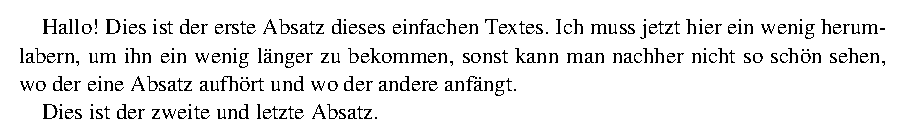
\includegraphics[width=\erstesdokumentbreite]{erstes-dokument}}
  \caption{Das Druckergebnis des ersten Dokumentes.}
  \label{fig:erstes-dokument}
\end{figure}

Zur Pr�ambel zun�chst nur Folgendes:

Die Zeilen~\ref{lst:start-pakete}--\ref{lst:helvet} sagen \LaTeX{} unter
anderem, dass wir Windows benutzen, und stellen die Schriftarten ein.

In Zeile~\ref{lst:ngerman} stelle ich die Sprache ein, "`ngerman"' steht f�r
"`deutsch --~neue Rechtschreibung"'.  Schlie�lich folgt der eigentliche Text,
zwischen \lstinline|\begin{document}| und \lstinline|\end{document}|.

Auch dieses Dokument kann man sich mit \keystroke{Strg}+\keystroke{F7}
und~\keystroke{F5} mal anschauen.  Das Ergebnis sieht man in
Abbildung~\vref{fig:erstes-dokument}.


\subsection{Wichtige grunds�tzliche \LaTeX-Regeln}

\begin{itemize}
\item Es spielt keine Rolle, ob man W�rter durch ein, zwei, oder wieviel
  Leerschritte auch immer trennt.  Im Ausdruck f�gt \LaTeX{} immer den
  korrekten Zwischenraum ein.
\item Abs�tze werden durch Leerzeilen voneinander getrennt.  Auch hier ist die
  Anzahl unwichtig.
\item Der Zeilenumbruch wird erst f�r den Ausdruck von \LaTeX{} berechnet.  Wie
  man den Text im Editor auf die Zeilen aufteilt, ist also egal.
\item Prozentzeichen~"`\verb|%|"' werden von \LaTeX{} nicht ausgedruckt, ebenso
  wie alles, was hinter dem~"`\verb|%|"' in der Zeile steht.  Man kann so
  Notizen einf�gen.  (Ein richtiges Prozentzeichen muss man als "`\verb|\%|"'
  eingeben.)
\end{itemize}



%       $Id: yap.tex,v 1.8 2005/06/28 14:20:34 bronger Exp $    
%
%     yap.tex -- Part of the LaTeX Tutorium
%     Copyright 2004 Project Members of
%                    https://github.com/latextemplates/latex-tutorium/
%                    
%
%   This program is free software; you can redistribute it and/or
%   modify it under the terms of the Artistic License 2.0 as published
%   by Larry Wall.  You should have received a copy of the Artistic
%   License 2.0 along with this program in the file COPYING; if not,
%   you can get it at
%     http://dev.perl.org/rfc/346.html
%   or contact the current maintainers of the LaTeX Tutorium.
%
%   This program is distributed in the hope that it will be useful, but
%   WITHOUT ANY WARRANTY; without even the implied warranty of
%   MERCHANTABILITY or FITNESS FOR A PARTICULAR PURPOSE.  See the
%   Artistic License 2.0 for more details.
%
%   This file may only be distributed together with a copy of the LaTeX
%   Turorium.
%
%   The LaTeX Tutorium consists of all files listed in manifest.txt.


\subsection{Die Schnellvorschau}
\index{Yap}
\index{Schnellvorschau}

Wie schon in \ref{sec:ersteschritte} gesagt, ruft ein Druck auf
\keystroke{Strg}+\keystroke{F7} gefolgt von \keystroke{F5} die
\emph{Schnellvorschau} auf.  Auf dem Weg zum Ausdruck oder zur \PDF-Datei ist
es nur ein Zwischenformat, das sich aber hervorragend zum Kontrolllesen eignet,
da es schnell erstellt und angezeigt wird.

\NZB{Grafiken im YAP?}

%%% Local Variables: 
%%% mode: latex
%%% TeX-master: "latex-tutorium"
%%% End: 

%       $Id: acrobat.tex,v 1.3 2004/01/20 09:06:41 bronger Exp $    
%
%     acrobat.tex -- Part of the LaTeX Tutorium
%     Copyright 2004 Project Members of
%                    https://github.com/latextemplates/latex-tutorium/
%                    
%
%   This program is free software; you can redistribute it and/or
%   modify it under the terms of the Artistic License 2.0 as published
%   by Larry Wall.  You should have received a copy of the Artistic
%   License 2.0 along with this program in the file COPYING; if not,
%   you can get it at
%     http://dev.perl.org/rfc/346.html
%   or contact the current maintainers of the LaTeX Tutorium.
%
%   This program is distributed in the hope that it will be useful, but
%   WITHOUT ANY WARRANTY; without even the implied warranty of
%   MERCHANTABILITY or FITNESS FOR A PARTICULAR PURPOSE.  See the
%   Artistic License 2.0 for more details.
%
%   This file may only be distributed together with a copy of the LaTeX
%   Turorium.
%
%   The LaTeX Tutorium consists of all files listed in manifest.txt.

\subsection{Endg�ltige Vorschau \& Drucken}

\begingroup\sffamily
PDF-Erzeugung (pdflatex), Acrobat-Reader

An dieser Stelle hyperref erw�hnen.
\endgroup

%%% Local Variables: 
%%% mode: latex
%%% TeX-master: "latex-tutorium"
%%% End: 

%       $Id: fehler.tex,v 1.3 2004/01/20 09:06:41 bronger Exp $    
%
%     fehler.tex -- Part of the LaTeX Tutorium
%     Copyright 2004 Project Members of
%                    https://github.com/latextemplates/latex-tutorium/
%                    
%
%   This program is free software; you can redistribute it and/or
%   modify it under the terms of the Artistic License 2.0 as published
%   by Larry Wall.  You should have received a copy of the Artistic
%   License 2.0 along with this program in the file COPYING; if not,
%   you can get it at
%     http://dev.perl.org/rfc/346.html
%   or contact the current maintainers of the LaTeX Tutorium.
%
%   This program is distributed in the hope that it will be useful, but
%   WITHOUT ANY WARRANTY; without even the implied warranty of
%   MERCHANTABILITY or FITNESS FOR A PARTICULAR PURPOSE.  See the
%   Artistic License 2.0 for more details.
%
%   This file may only be distributed together with a copy of the LaTeX
%   Turorium.
%
%   The LaTeX Tutorium consists of all files listed in manifest.txt.


\subsection{Wenn mal was schiefgeht~\dots}

\begingroup\sffamily
Typische Probleme:
\begin{itemize}
\item \LaTeX-Kompilierfehler
\item Probleme mit dem Editor (Undo u.�.)
\end{itemize}
(Probleme mit Grafiken werden dort behandelt.)
\endgroup

%%% Local Variables: 
%%% mode: latex
%%% TeX-master: "latex-tutorium"
%%% End: 


%%% Local Variables: 
%%% mode: latex
%%% TeX-master: "latex-tutorium"
%%% End: 

% LocalWords:  Strg document numbers left basicstyle herumlabern fig dokument
% LocalWords:  ngerman


%       $Id: gliederung.tex,v 1.13 2005/06/28 18:30:35 bronger Exp $    
%
%     gliederung.tex -- Part of the LaTeX Tutorium
%     Copyright 2004 Project Members of
%                    https://github.com/latextemplates/latex-tutorium/
%                    
%
%   This program is free software; you can redistribute it and/or
%   modify it under the terms of the Artistic License 2.0 as published
%   by Larry Wall.  You should have received a copy of the Artistic
%   License 2.0 along with this program in the file COPYING; if not,
%   you can get it at
%     http://dev.perl.org/rfc/346.html
%   or contact the current maintainers of the LaTeX Tutorium.
%
%   This program is distributed in the hope that it will be useful, but
%   WITHOUT ANY WARRANTY; without even the implied warranty of
%   MERCHANTABILITY or FITNESS FOR A PARTICULAR PURPOSE.  See the
%   Artistic License 2.0 for more details.
%
%   This file may only be distributed together with a copy of the LaTeX
%   Turorium.
%
%   The LaTeX Tutorium consists of all files listed in manifest.txt.


\section{Gliederung des Textes}

\subsection{Titel und Autor}

Wenn man einen Titel und/oder einen Autor f�r das Dokument angeben m�chte, muss
man das in Form von
\begin{lstlisting}
\title{Der Herr der Ringe}
\author{J.R.R. Tolkien}
\end{lstlisting}
unmittelbar nach dem \lstinline|\begin{document}| tun.  Im Dokument gibt man
mit \lstinline{\maketitle} an, wo man den Titel hinhaben m�chte.  Meist ist das
nat�rlich ganz vorne:
\begin{lstlisting}
\begin{document}
\title{Der Herr der Ringe}
\author{J.R.R. Tolkien}
\maketitle
...
\end{lstlisting}


\subsection{Kapitel, Abschnitte und das Inhaltsverzeichnis}

Ein neues Kapitel oder ein neuer Abschnitt beginnt immer mit einer �berschrift.
Daf�r muss man einen der Befehle benutzen, die in
Tabelle~\vref{tab:Gliederungs-Befehle} aufgelistet sind.  Man kann also
beispielsweise schreiben:
\begin{lstlisting}
\section{Einf�hrung}

In diesem Artikel werde ich erkl�ren, wie ...
\end{lstlisting}

\begin{table}
  \caption{\LaTeX-Befehle, mit denen man �berschriften einf�gt.}
  \label{tab:Gliederungs-Befehle}
  \vspace{1ex}
  \centering
  \begin{tabular}{@{}ll@{}}
    \toprule
    \verb|\chapter{|\emph{�berschrift}\verb|}|        &  Kapitel (nur in B�chern)  \\
    \verb|\section{|\emph{�berschrift}\verb|}|        &  Abschnitte                \\
    \verb|\subsection{|\emph{�berschrift}\verb|}|     &  Unterabschnitte           \\
    \verb|\subsubsection{|\emph{�berschrift}\verb|}|  &  Unter-Unterabschnitte     \\
    \bottomrule
  \end{tabular}
\end{table}

\begin{wrapfigure}{r}{5cm}
  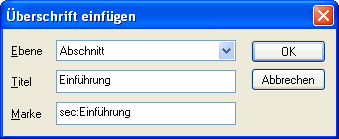
\includegraphics{ueberschriften}
\end{wrapfigure}
Man kann es sich aber auch etwas bequemer machen.  Mit \Alt+\Ctrl+\keystroke S
wird ein Fenster ge�ffnet, in dem man w�hlen kann, was f�r eine Art von
�berschrift man einf�gen m�chte, wie die �berschrift lauten soll und welche
Marke man hier setzen m�chte (siehe Abschnitt~\vref{sec:Querverweise}).

Dort, wo man den Befehl \lstinline{\tableofcontents} einf�gt, druckt \LaTeX{}
ein Inhaltsverzeichnis.  Ein typischer Start f�r ein \LaTeX-Dokument ist daher
\begin{lstlisting}
\begin{document}
\title{Der Herr der Ringe}
\author{J.R.R. Tolkien}
\maketitle
\tableofcontents
...
\end{lstlisting}


\subsection{Querverweise}
\label{sec:Querverweise}

Es w�re ziemlich dumm, direkt eine Nummer einzuf�gen, wenn man auf einen
anderen Abschnitt, eine bestimmte Seite, eine Tabelle, Grafik oder �hnliches
verweisen m�chte.  Der Grund ist einfach, dass sich die Nummern sehr leicht
�ndern, wenn man den Text bearbeitet.

In \LaTeX{} setzt man daher mit dem Befehl \lstinline{\label} sogenannte
\emph{Marken} (engl.~"`labels"') an die Stellen, auf die man verweisen m�chte
(meist direkt dahinter).  Dabei vergibt man einen eindeutigen Namen f�r die
Marke.

Wie im vorangehenden Abschnitt schon beschrieben, kann man gleich bei der
Eingabe einer �berschrift eine Marke setzen.  Es ist �blich, Marken f�r
�berschriften mit "`sec:"'\ zu beginnen.  Mal angenommen, ich habe die folgende
�berschrift:
\begin{lstlisting}
\section{Einf�hrung}
\label{sec:Einf�hrung}
\end{lstlisting}
Dann kann ich an einer beliebigen Stelle im Dokument auf diese �berschrift mit
\lstinline{\ref} und \lstinline{\pageref} verweisen:
\begin{lstlisting}
...  Siehe Abschnitt \ref{sec:Einf�hrung} auf
Seite \pageref{sec:Einf�hrung}.  ...
\end{lstlisting}
\LaTeX{} ersetzt \lstinline|\ref{|\dots\lstinline|}| durch die
Abschnitts-Nummer und \lstinline|\pageref{|\dots\lstinline|}| durch die
Seitenzahl.

\nopagebreak
Genauso kann man auch auf Tabellen, Grafiken, Formeln oder beliebige Positionen
im Text verweisen.


\subsection{Listen und Aufz�hlungen}

In \LaTeX{} werden Listen als Umgebungen eingegeben.  Es gibt drei Arten von
Listen: Normale Listen (itemize), Aufz�hlungen (enumerate) und
Begriffs-Erkl�rungen (description).

\begingroup
\newcommand{\mycolumnwidth}{}
\newdimen\mycolumnwidth\mycolumnwidth\hsize\advance\mycolumnwidth-\parindent
\mycolumnwidth0.5\mycolumnwidth
\begin{tabular}{@{}p{\mycolumnwidth}@{}p{\mycolumnwidth}@{}}
Normale Listen sehen so aus:
\begin{itemize}
\item Punkt Eins
\item Punkt Zwei
\item Punkt Drei
\end{itemize}
&
und werden so eingegeben:
%
\begin{lstlisting}
\begin{itemize}
\item Punkt Eins
\item Punkt Zwei
\item Punkt Drei
\end{itemize}
\end{lstlisting}
\end{tabular}
\endgroup

Mit einer Aufz�hlung ist Folgendes gemeint:
\begin{enumerate}
\item Punkt Eins
\item Punkt Zwei
\item Punkt Drei
\end{enumerate}
Das gibt man genauso wie Listen ein, nur schreibt man statt "`\verb|itemize|"'
"`\verb|enumerate|"'.

\medskip
Schlie�lich kann man noch Begriffe in einer Liste erkl�ren:
\begin{description}
\item[Asterix,] der Held dieser Abenteuer.  Ein listiger kleiner Krieger, voll
  spr�hender Intelligenz, dem alle gef�hrlichen Auftr�ge bedenkenlos anvertraut
  werden.  \dots
\item[Obelix] ist der dickste Freund von Asterix.  Seines Zeichens Lieferant
  f�r Hinkelsteine, gro�er Liebhaber von Wildschweinen und \dots
\item[Miraculix,] der ehrw�rdige Druide des Dorfes, schneidet Misteln und braut
  Zaubertr�nke.  \dots
\end{description}
%
Daf�r muss man die description-Umgebung benutzen und den zu erkl�renden Begriff
in eckigen Klammern hinter das \lstinline{\item} setzen:
%
\begin{lstlisting}[basicstyle=\ttfamily\ifminion\else\footnotesize\fi]
\begin{description}
\item[Asterix,] der Held dieser Abenteuer.  Ein listiger
  kleiner Krieger, voll spr�hender Intelligenz, dem alle
  gef�hrlichen Auftr�ge bedenkenlos anvertraut werden.
  \dots{}
\item[Obelix] ist der dickste Freund von Asterix.  Seines
  Zeichens Lieferant f�r Hinkelsteine, gro�er Liebhaber
  von Wildschweinen und \dots{}
...
\end{description}
\end{lstlisting}


%%% Local Variables: 
%%% mode: latex
%%% TeX-master: "latex-tutorium"
%%% End: 


%       $Id: formatierung.tex,v 1.19 2005/06/28 18:30:35 bronger Exp $    
%
%     formatierung.tex -- Part of the LaTeX Tutorium
%     Copyright 2004 Project Members of
%                    http://sourceforge.net/projects/latex-tutorium/
%                    
%
%   This program is free software; you can redistribute it and/or
%   modify it under the terms of the Artistic License 2.0 as published
%   by Larry Wall.  You should have received a copy of the Artistic
%   License 2.0 along with this program in the file COPYING; if not,
%   you can get it at
%     http://dev.perl.org/rfc/346.html
%   or contact the current maintainers of the LaTeX Tutorium.
%
%   This program is distributed in the hope that it will be useful, but
%   WITHOUT ANY WARRANTY; without even the implied warranty of
%   MERCHANTABILITY or FITNESS FOR A PARTICULAR PURPOSE.  See the
%   Artistic License 2.0 for more details.
%
%   This file may only be distributed together with a copy of the LaTeX
%   Turorium.
%
%   The LaTeX Tutorium consists of all files listed in manifest.txt.


\section{Formatierung}

\subsection{Fett, kursiv etc}

\begin{table}[htbp]
  \caption{Einige M�glichkeiten der Textformatierung}
  \label{tab:Auszeichnungen}
  \vspace{1ex}
  \centering
  \begin{tabular}{@{}lcc@{}}
    \toprule
    Formatierung              &  Tastenk�rzel        &  Beispiel                   \\
    \midrule
    \emph{kursiv}             &  \Ctrl+\keystroke E  &  \lstinline|\emph{Wort}|    \\
    \textbf{fett}             &                      &  \lstinline|\textbf{Wort}|  \\
    \textsc{Kapit�lchen}      &                      &  \lstinline|\textsc{Wort}|  \\
    \textsf{serifenlos}       &                      &  \lstinline|\textsf{Wort}|  \\
    \texttt{Schreibmaschine}  &                      &  \lstinline|\texttt{Wort}|  \\
    \bottomrule
  \end{tabular}
\end{table}

Wenn man ein Wort oder einen Satz betonen m�chte, druckt man ihn am besten
\emph{kursiv}.  Das geht mit \Ctrl+\mbox{\keystroke E,} welches den Befehl
\lstinline{\emph} (engl.~\emph{emphasize}--\emph{betonen}) einf�gt:
\begin{lstlisting}
... druckt man ihn am besten \emph{kursiv}.
\end{lstlisting}
In den allermeisten Texten kommt man mit Kursivdruck aus.  Trotzdem sind in
Tabelle~\vref{tab:Auszeichnungen} noch weitere M�glichkeiten aufgelistet.  Man
kann sie auch kombinieren:
\begin{lstlisting}
\textbf{\emph{fett-kursiv}}
\end{lstlisting}


\begin{table}[t]
  \caption{Einige Schriftarten-Befehle.}
  \label{tab:Schriftarten}
  \vspace{1ex}
  \newcommand{\tone}{\fontencoding{OT1}}
  \centering\small
  \begin{tabular}{@{}lll@{}}
    \toprule
    Befehl & Schriftart & wirkt auf\\
    \midrule
    \verb|\usepackage{mathptmx}| & \fontfamily{ptm}\selectfont Times New Roman & Normaltext \& Formeln \\
    \verb|\usepackage{mathpazo}| & \fontfamily{ppl}\selectfont Palatino        & Normaltext \& Formeln \\
    \verb|\usepackage{courier}|  & \fontfamily{pcr}\selectfont Courier         & Text in Schreib-\\
                                 &                 & \quad maschinenschrift \\
    \multicolumn{2}{@{}l}{\texttt{\textbackslash usepackage[scaled]\char'173 helvet\char'175}} & \\
    & \fontfamily{phv}\selectfont Helvetica & Serifenloser Text      \\
    \verb|\usepackage{bookman}|  & \fontfamily{pbk}\selectfont Bookman         & Normaltext             \\
    \verb|\usepackage{newcent}|  & \fontfamily{pnc}\selectfont New Century     & Normaltext             \\
                                 & \quad\fontfamily{pnc}\selectfont Schoolbook&                        \\
    \verb|\usepackage{avant}|    & \fontfamily{pag}\selectfont Avant Garde     & serifenlosen Text      \\
    \verb|\usepackage{charter}|  & \fontfamily{bch}\selectfont Charter         & Normaltext             \\
    \verb|\usepackage{chancery}| & \fontfamily{pzc}\selectfont Zapf Chancery   & Normaltext             \\
    \emph{(Voreinstellung)}      & \fontfamily{cmr}\tone\selectfont Computer Modern & Normaltext \& Formeln  \\
    \emph{(Voreinstellung)}      & \fontfamily{cmss}\tone\selectfont CM Sans Serif  & serifenlosen Text      \\
    \emph{(Voreinstellung)}      & \fontfamily{cmtt}\tone\selectfont CM Typewriter  & Text in Schreib-       \\
                                 &                 & \quad maschinenschrift \\
    \bottomrule
  \end{tabular}
\end{table}

\subsection{Schriftarten}

Es ist m�glich, nahezu jede beliebige Schriftart, die man besitzt, mit \LaTeX{}
zu benutzen.  Da \LaTeX{} sehr viele Informationen �ber Schriftarten ben�tigt,
ist das aber viel Arbeit.  Gl�cklicherweise haben sich bereits andere diese
M�he gemacht, zumindest f�r die interessanten Schriftarten.

Die Beispiele in diesem Tutorium werden in "`Times New Roman"' gedruckt, die
Schriftart, die meist mit Word benutzt wird.  Wenn man sich nochmal das
Muster-Dokument auf Seite~\pageref{Minimaldokument} anschaut, sieht man dort in
den Zeilen~\ref{lst:mathptmx-courier} und~\ref{lst:helvet}
\begin{lstlisting}
\usepackage{mathptmx,courier}
\usepackage[scaled]{helvet}
\end{lstlisting}
Diese kryptischen Befehle stellen auf Times (f�r normaler Text \& Formeln),
Courier (f�r Schreibmaschinen-Schrift) und Helvetica (f�r serifenlos).

Will man andere Schriftarten haben, muss man diese Zeilen l�schen und einen
oder mehrere der in Tabelle~\vref{tab:Schriftarten} genannten Schriftartbefehle
an dieser Stelle einf�gen.


\subsection{Besondere Textsymbole, Trennungen und Leerr�ume}
\label{sec:sonderzeichen}

Einige Zeichen haben in \LaTeX{} eine besondere Bedeutung.  Wir hatten
beispielsweise schon gesehen, dass das Prozent-Zeichen bewirkt, dass der Rest
der Zeile ignoriert wird.  Was aber, wenn man wirklich ein Prozent-Zeichen
eingeben m�chte?

In diesem Fall muss man einfach einen Backslash~``\verb|\|'' davorstellen.  Man
kann also schreiben
\begin{lstlisting}
Die SPD kam auf 33,3\%.
\end{lstlisting}
Das gilt ebenso f�r die Zeichen \&, \# und~\$.

Zwei Bindestriche ``\verb|--|'' f�gen einen Gedankenstrich ein -- den man auch
f�r von-bis-Ausdr�cke verwenden kann: Von 14--15~Uhr.  Achtung, das ist kein
Bindestrich!  Der ist weiterhin blo� ein einzelnes~``\verb|-|''.

Die "`G�nsef��chen"' m�ssen in \LaTeX{} etwas seltsam eingegeben werden:
\begin{lstlisting}
Ein sogenannter "`Roter Riese"' ist ein
Stern, der ...
\end{lstlisting}
allerdings erledigt das der Editor bereits automatisch.

\begin{table}
  \caption{Besondere Zeichen in \LaTeX{}}
  \label{tab:Sonderzeichen}
  \vspace{1ex}
  \centering
  \begin{tabular}{@{}lcl@{}}
    \toprule
    \LaTeX-Befehl  &  Aussehen  &  Beschreibung \\
    \midrule
    \verb|\&|, \verb|\$|, \verb|\%|, \verb|\#| & \&, \$, \%, \# & \\
    \verb|\S{}|  & \S{}  &  Paragraphen-Zeichen \\
    \verb|--|  &  --  &  Gedankenstrich, von--bis-Strich \\
    \verb|\dots{}|  &  \dots  &  Auslassungspunkte \\
    \verb|"`|\dots\verb|"'|  &  "`\dots"'  &  G�nsef��chen \\
    \verb|~|   &      &  Leerschritt, Zeilenumbruch verboten \\
    \verb|\,|   &     &  halber Leerschritt, Zeilenumbruch \\
                &          &  \quad verboten \\
    \verb|"~|  &  -   &  Bindestrich, Zeilenumbruch verboten \\
%    \verb|""|  &  (\emph{nichts})    &  Zeilenumbruch erlaubt, keinen \\
%               &                     &  \quad Bindestrich einf�gen \\
    \verb|\LaTeX{}|  &  \LaTeX{}  &  offizielles \LaTeX-Logo \\
    \bottomrule
  \end{tabular}
\end{table}
Ach ja, last but not least: "`\LaTeX{}"' schreibt man "`\lstinline|\LaTeX{}|"'.

\bigskip\noindent
Manchmal will man die Silbentrennung oder den Zeilenumbruch beeinflussen.  Da
bietet \LaTeX{} einfache und praktische M�glichkeiten.  Eine Tilde ``\verb|~|''
beispielsweise erzeugt ein Leerzeichen, an dem nie ein Zeilenumbruch
stattfindet:
\begin{lstlisting}
Die Pr�fung leitet Prof.~Dr.~Obermeyer.
\end{lstlisting}
Dasselbe verursacht ein ``\verb|\,|'', allerdings ist das nur ein halbes
Leerzeichen:
\begin{lstlisting}
Er war 175\,cm gro�.
\end{lstlisting}
Wenn ich einen Bindestrich brauche, an dem nie die Zeile umbrochen werden darf,
gebe ich ihn mit \verb|"~| ein:
\begin{lstlisting}
Seine Aussage im O"~Ton war, dass ...
Das gibt Abz�ge in der B"~Note.
\end{lstlisting}
So kann man garantieren, dass solche F�lle immer richtig getrennt werden.
Tabelle~\vref{tab:Sonderzeichen} enth�lt eine �bersicht �ber diese Befehle.

Falls einzelne W�rter falsch getrennt werden sollten, f�hrt man einfach alle
m�glichen Trennungen des Wortes in der Pr�ambel mit Hilfe des Befehls
\lstinline|\hyphenation| auf:
\begin{lstlisting}
\hyphenation{Text-ein-ga-be Zei-len-um-bruch}
\end{lstlisting}

%%% Local Variables: 
%%% mode: latex
%%% TeX-master: "latex-tutorium"
%%% End: 


%       $Id: grafiken.tex,v 1.11 2004/08/02 11:33:02 bronger Exp $    
%
%     grafiken.tex -- Part of the LaTeX Tutorium
%     Copyright 2004 Project Members of
%                    http://sourceforge.net/projects/latex-tutorium/
%                    
%
%   This program is free software; you can redistribute it and/or
%   modify it under the terms of the Artistic License 2.0 as published
%   by Larry Wall.  You should have received a copy of the Artistic
%   License 2.0 along with this program in the file COPYING; if not,
%   you can get it at
%     http://dev.perl.org/rfc/346.html
%   or contact the current maintainers of the LaTeX Tutorium.
%
%   This program is distributed in the hope that it will be useful, but
%   WITHOUT ANY WARRANTY; without even the implied warranty of
%   MERCHANTABILITY or FITNESS FOR A PARTICULAR PURPOSE.  See the
%   Artistic License 2.0 for more details.
%
%   This file may only be distributed together with a copy of the LaTeX
%   Turorium.
%
%   The LaTeX Tutorium consists of all files listed in manifest.txt.


\section{Grafiken}
\label{sec:Grafiken}

Grafiken werden mit dem Men�-Punkt "`Einf�gen--Grafik"' eingef�gt oder mit
\Alt+\Ctrl+\keystroke A (f�r "`Abbildung"').  Es �ffnet sich dann das
Dialogfenster von Abbildung~\vref{fig:Grafiken}.

\begin{figure}
  \centering
  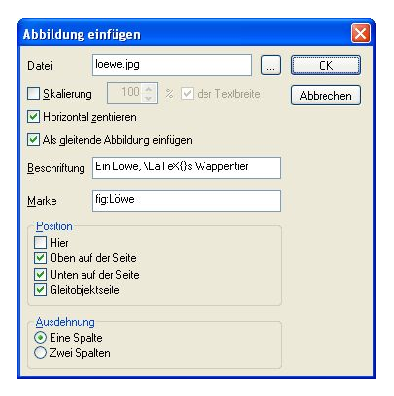
\includegraphics{abbildungen}
  \caption{Das Dialogfenster zum Einf�gen von Grafiken}
  \label{fig:Grafiken}
\end{figure}

Man gibt dort zuerst den Dateinamen der Bilddatei an.  Daf�r muss man die
Grafik aus dem Programm, mit dem man die Grafik erstellt hat (z.\,B. Corel
Draw, Photopaint, Excel oder die DigiCam-Software) erst einmal
\emph{exportieren}, damit man eine Datei erh�lt.  Das h�ngt stark vom Programm
ab, meist geht es �ber das Men� "`Datei--Exportieren"'.  Dann kann man f�r
gew�hnlich die Art der Grafikdatei w�hlen.


\subsection*{Einschub: Grunds�tzliches zu Bilddateien}

Es gibt viele Arten von Bilddateien; \LaTeX{} kann \JPEG"~, \PDF- und
\PNG-Dateien direkt in einen Text einbetten:
\begin{description}
\item[\JPEG] ist f�r Fotos und �hnliches gedacht.  Die Dateien
  haben meistens die Endung ``\verb|.jpg|''.
\item[\PDF] ist eigentlich ein Dateiformat f�r ganze Dokumente.  \LaTeX{}
  erzeugt am Ende ja selber ein \PDF\@.  Man kann aber auch einzelne Grafiken
  als \PDF{} abspeichern, z.\,B. mit Corel Draw oder Excel.  Wie das geht,
  steht in Anhang~\vref{sec:FreePDF-usage}\@.  Dieses Format sollte man f�r
  Diagramme oder schematische Zeichnungen benutzen.
\item[\PNG] schlie�lich ist auch f�r Zeichnungen geeignet, hat aber eine
  geringere Qualit�t als \PDF\@.  Es ist daher eher eine Notl�sung, oder f�r
  spezielle Zwecke.
\end{description}
Es gibt noch viele andere Arten von Bilddateien.  Sie m�ssen, damit sie mit
\LaTeX{} verwendbar sind, als \PDF{} abgespeichert werden (siehe wiederum
Anhang~\ref{sec:FreePDF-usage})\@.

\nopagebreak
\noindent\hbox to \linewidth{\large\itshape\hfill Einschub Ende}
\bigskip

\begin{figure}
  \centering
  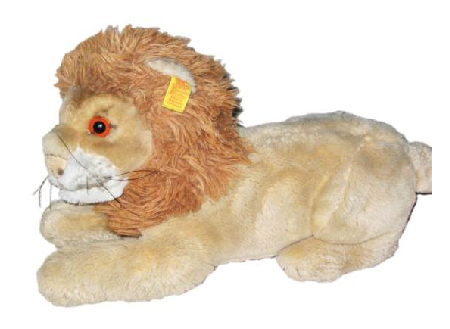
\includegraphics{loewe}
  \caption{Ein L�we, \LaTeX{}s Wappentier}
  \label{fig:L�we}
\end{figure}

\noindent
Wenn man die Bilddatei angegeben hat, kann man noch eine Bildunterschrift und
eventuell eine Marke eingeben (f�r Querverweise, siehe
Seite~\pageref{sec:Querverweise}), und dann auf "`OK"' dr�cken.  Der Editor
f�gt dann die notwendigen Befehle in den Text ein:
\begin{lstlisting}
\begin{figure}
  \centering
  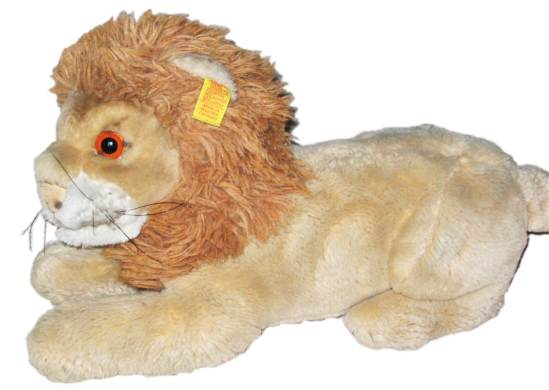
\includegraphics{loewe.jpg}
  \caption{Ein L�we, \LaTeX{}s Wappentier}
  \label{fig:L�we}
\end{figure}
\end{lstlisting}
Das Ergebnis sieht man in Abbildung~\vref{fig:L�we}.


\subsection{Gleitende und nicht-gleitende Abbildungen}
\label{sec:Gleitobjekte}

Was wir gerade eingef�gt haben, war eine sogenannte \emph{gleitende Abbildung}.
Das ist eine Abbildung, f�r die \LaTeX{} den passenden Ort selber sucht.  Man
kann dieses Verhalten auch beeinflussen, daf�r sind die Felder unter
"`Position"' in der Dialogbox da.  Alles, was man dort markiert, sind erlaubte
Positionen f�r die Abbildung.

\begin{wrapfigure}{r}{5cm}
  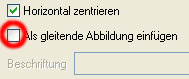
\includegraphics{tabelle1}
\end{wrapfigure}
Eine gleitende Abbildung ist zwar etwas ungemein praktisches, und in den
meisten F�llen nutzt man das auch.  Aber manchmal will man einfach nur eine
Grafik an der aktuellen Position im Text haben.  Dann muss man die Option "`Als
gleitende Abbildung einf�gen"' abw�hlen.  Allerdings ist es dann nicht mehr
m�glich, eine Bildunterschrift zu setzen.


%%% Local Variables: 
%%% mode: latex
%%% TeX-master: "latex-tutorium"
%%% End: 


%       $Id: tabellen.tex,v 1.13 2004/05/23 10:56:44 bronger Exp $    
%
%     tabellen.tex -- Part of the LaTeX Tutorium
%     Copyright 2004 Project Members of
%                    https://github.com/latextemplates/latex-tutorium/
%                    
%
%   This program is free software; you can redistribute it and/or
%   modify it under the terms of the Artistic License 2.0 as published
%   by Larry Wall.  You should have received a copy of the Artistic
%   License 2.0 along with this program in the file COPYING; if not,
%   you can get it at
%     http://dev.perl.org/rfc/346.html
%   or contact the current maintainers of the LaTeX Tutorium.
%
%   This program is distributed in the hope that it will be useful, but
%   WITHOUT ANY WARRANTY; without even the implied warranty of
%   MERCHANTABILITY or FITNESS FOR A PARTICULAR PURPOSE.  See the
%   Artistic License 2.0 for more details.
%
%   This file may only be distributed together with a copy of the LaTeX
%   Turorium.
%
%   The LaTeX Tutorium consists of all files listed in manifest.txt.

\section{Tabellen}

Um eine Tabelle einzuf�gen, sind drei Schritte notwendig.
\begin{enumerate}
\item Im Men� "`Einf�gen--Tabelle"' w�hlen.  Entscheiden, ob die Tabelle
  "`gleiten"' soll oder nicht (s.\,u.).  Als Ergebnis wird eine leere
  Rumpf-Tabelle in das Dokument eingef�gt.
\item Die Zahl der Spalten und die Spalten-Ausrichtung angeben.
\item Die Zeilen und Spalten der Tabelle eingeben.
\end{enumerate}

Betrachten wir die folgende Beispiel-Tabelle:
\begin{center}
  \begin{tabular}{llc}
    \toprule
    Sternname   &  Sternbild  &  Entfernung (Lj) \\
    \midrule
    Rigel       &  Orion      &     780          \\
    Acturus     &  Bo�tes     &      37          \\
    Deneb       &  Schwan     &    3200          \\
    Rigil Kent  &  Zentaur    &      4,4         \\
    \bottomrule             
  \end{tabular}
\end{center}

\begin{figure}
  \centering
  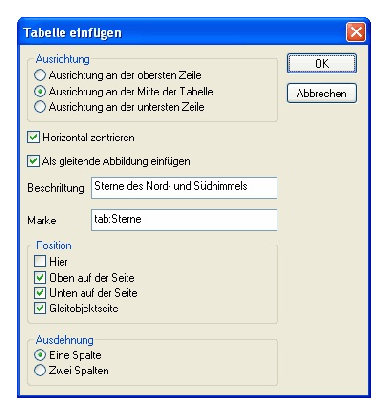
\includegraphics{tabelle2}
  \caption{Einf�gen einer gleitenden Tabelle}
  \label{fig:Gleittabelle}
\end{figure}

Um das einzugeben, w�hlt man im Men� "`Einf�gen--Tabelle"' oder dr�ckt
\Alt+\Ctrl+\mbox{\keystroke T\@.}  Es �ffnet sich das Dialog-Fenster in
Abbildung~\ref{fig:Gleittabelle}.  Dort kann man noch eine Beschriftung und
eine Marke eingeben (f�r Querverweise, siehe Seite~\pageref{sec:Querverweise}),
und muss auf "`OK"' dr�cken.  Der Editor f�gt dann automatisch eine Art Rumpf
f�r die Tabelle ein:
\begin{lstlisting}[escapeinside=`']
\begin{table}
  \centering
  \begin{tabular}
    `\textrm{\emph{(Hier stehen die Zeilen und Spalten)}}'
  \end{tabular}
  \caption{Sterne des Nord- und S�dhimmels}
  \label{tab:Sterne}
\end{table}
\end{lstlisting}
Als n�chstes m�ssen wir \LaTeX{} sagen, wieviele Spalten unsere Tabelle haben
soll.  In unserem Fall sind es offensichtlich drei.  Also schreibe ich ein
"`\lstinline|{llc}|"' hinter das \lstinline|\begin{tabular}|:
\begin{lstlisting}
  ...
  \begin{tabular}{llc}
    ...
\end{lstlisting}
Jeder der drei Buchstaben steht f�r eine Spalte.  Ein "`l"' bedeutet
\emph{linksb�ndige} Ausrichtung.  Entsprechend stehen "`r"' und "`c"' fuer
\emph{rechtsb�ndig} und \emph{zentriert}.  F�r unser Beispiel sollen also die
ersten beiden Spalten links ausgerichtet werden, und die letzte zentriert.

Jetzt kann man die Tabelle mit Inhalt f�llen.  Tabellen werden zeilenweise
eingegeben.  Spalten trennt man mit "`\&"'"~Zei\-chen, Zeilen m�ssen mit
"`\verb|\\|"' beendet werden:
\begin{lstlisting}[basicstyle=\ttfamily\ifminion\else\footnotesize\fi]
  ...
  \begin{tabular}{llc}
    \toprule
    Sternname   &  Sternbild  &  Entfernung (Lj) \\
    \midrule
    Rigel       &  Orion      &     780          \\
    Acturus     &  Bo�tes     &      37          \\
    Deneb       &  Schwan     &    3200          \\
    Rigil Kent  &  Zentaur    &      4,4         \\
    \bottomrule             
  \end{tabular}
  ...
\end{lstlisting}
\lstinline{\toprule}, \lstinline{\midrule} und \lstinline{\bottomrule} erzeugen
die obere, mittlere und untere Linie in der Tabelle.

\begin{table}
  \centering
  \begin{tabular}{llc}
    \toprule
    Sternname   &  Sternbild  &  Entfernung (Lj) \\
    \midrule
    Rigel       &  Orion      &     780          \\
    Acturus     &  Bo�tes     &      37          \\
    Deneb       &  Schwan     &    3200          \\
    Rigil Kent  &  Zentaur    &      4,4         \\
    \bottomrule             
  \end{tabular}
  \caption{Sterne des Nord- und S�dhimmels}
  \label{tab:Sterne}
\end{table}

\nopagebreak
Das Ergebnis sieht man in Tabelle~\vref{tab:Sterne}.  Tabellen sind in \LaTeX{}
am Anfang etwas einsch�chternd, aber man gew�hnt sich recht schnell daran.


\subsection{Gleitende und nicht-gleitende Tabellen}
\label{sec:Gleittabellen}

Genauso wie auch bei Abbildungen gibt es \emph{gleitende} und
\emph{nicht-gleitende} Tabellen.  Wir haben oben eine gleitende Tabelle
eingef�gt, d.\,h.\ sie kann eine Beschriftung haben, und \LaTeX{} sucht
selbstst�ndig den besten Platz f�r sie.  Das ganze ist v�llig analog zu
Abbildungen, siehe Abschnitt~\vref{sec:Gleitobjekte}.


%%% Local Variables: 
%%% mode: latex
%%% TeX-master: "latex-tutorium"
%%% End: 


%       $Id: fortgeschrittenes.tex,v 1.11 2005/06/28 18:30:35 bronger Exp $    
%
%     fortgeschrittenes.tex -- Part of the LaTeX Tutorium
%     Copyright 2004 Project Members of
%                    http://sourceforge.net/projects/latex-tutorium/
%                    
%
%   This program is free software; you can redistribute it and/or
%   modify it under the terms of the Artistic License 2.0 as published
%   by Larry Wall.  You should have received a copy of the Artistic
%   License 2.0 along with this program in the file COPYING; if not,
%   you can get it at
%     http://dev.perl.org/rfc/346.html
%   or contact the current maintainers of the LaTeX Tutorium.
%
%   This program is distributed in the hope that it will be useful, but
%   WITHOUT ANY WARRANTY; without even the implied warranty of
%   MERCHANTABILITY or FITNESS FOR A PARTICULAR PURPOSE.  See the
%   Artistic License 2.0 for more details.
%
%   This file may only be distributed together with a copy of the LaTeX
%   Turorium.
%
%   The LaTeX Tutorium consists of all files listed in manifest.txt.


\section{Fortgeschrittenes Layout}

\minisec{Fu�noten}

Fu�noten werden mit \Alt+\Ctrl+\keystroke F erzeugt.  Diese Tastenkombination
f�gt den Befehl
\begin{lstlisting}
\footnote{}
\end{lstlisting}
ein.  Zwischen die geschweiften Klammern schreibt man dann den Text, der zur
Fu�note werden soll:\footnote{So wie hier}
\begin{lstlisting}
... werden soll:\footnote{So wie hier}
\end{lstlisting}

\minisec{Links ins Internet}

Internet-Adressen schreibt man mit dem Befehl \lstinline{\url}, der vom Paket
\Package{url} bereit gestellt wird (die Einbindung erkl�rt Abschnitt
\vref{sec:pakete}).
\begin{lstlisting}
Die Homepage der RWTH Aachen ist
\url{http://www.rwth-aachen.de}.
\end{lstlisting}
Im \PDF-Dokument sind diese Links nat�rlich anklickbar.


\subsection{Seitenr�nder einstellen}

\begin{table}
  \caption{Optionen zum Einstellen der Seitenr�nder}
  \label{tab:Seitenraender}
  \vspace{1ex}
  \centering
  \begin{tabular}{@{}ll@{}}
    \toprule
    K�rzel  &  Beschreibung \\
    \midrule
    a$5$paper      &  Papierformat auf A$5$ einstellen \\
    left=$X$cm     &  linken Rand auf $X$\,cm einstellen \\
    right=$X$cm    &  rechten Rand auf $X$\,cm einstellen \\
    top=$X$cm      &  oberen Rand auf $X$\,cm einstellen \\
    bottom=$X$cm   &  unteren Rand auf $X$\,cm einstellen \\
    \bottomrule
  \end{tabular}
\end{table}

Seitenr�nder werden in \LaTeX{} am besten mit dem Befehl
\begin{lstlisting}
\usepackage[...]{geometry}
\end{lstlisting}
eingestellt.  Dieser Befehl muss irgendwo in der Pr�ambel vor dem
\lstinline|\begin{document}| kommen.  Zwischen die eckigen Klammern schreibt
  man dann, wie man die Seitenr�nder gerne h�tte, zum Beispiel:
\begin{lstlisting}
\usepackage[a5paper,
  left=1.9cm, right=2.1cm,
  top=1.2cm, bottom=2.3cm]{geometry}
\end{lstlisting}
Das stellt auf \versalien{DIN}\,A$5$-Papier ein, und setzt die vier R�nder auf
die angegebenen Werte in Zenimentern.  Die Tabelle~\vref{tab:Seitenraender}
listet die wichtigsten Optionen f�r die Seiten-Einstellung auf.  (Es gibt
allerdings noch mehr, z.\,B. f�r Kopf- und Fu�zeilen.)


\subsection{Andere Sprachen}

\begin{table}
  \caption{Beispiele f�r Sprachen bei \LaTeX{}}
  \label{tab:Sprachen}
  \vspace{1ex}
  \centering
  \begin{tabular}{@{}ll@{}}
    \toprule
    english             &  amerikanisches Englisch \emph{(Voreinstellung)}  \\
    UKenglish           &  britisches Englisch                              \\
    german              &  Deutsch, Alte Rechtschreibung                    \\
    ngerman             &  Deutsch, Neue Rechtschreibung                    \\
    french              &  Franz�sisch                                      \\
    \bottomrule
  \end{tabular}
\end{table}

Wenn man nichts anderes sagt, geht \LaTeX{} davon aus, dass man einen Text auf
Englisch schreibt.  Werfen wir nochmal einen Blick auf das Beispiel auf
Seite~\pageref{lst:ngerman}, und zwar auf die Zeile~\ref{lst:ngerman}:
\begin{lstlisting}
\usepackage[ngerman]{babel}
\end{lstlisting}
Diese Zeile stellt die Sprache auf "`Deutsch -- Neue Rechtschreibung"' ein.
Falls man statt "`ngerman"' einfach nur "`german"' schreibt, werden alte
Rechtschreibregeln angewandt.  Tabelle~\vref{tab:Sprachen} listet ein paar
Sprachk�rzel auf, die man zwischen die eckigen Klammern schreiben kann.  Aber
es gibt ebenso "`italian"', "`dutch"', "`spanish"' und noch viele weitere, auch
f�r nicht-lateinische Schriften.

�brigens hat diese Einstellung nur Auswirkungen auf den \emph{Druck} des
Textes, insbesondere auf die korrekte Silbentrennung.  Die
\emph{Rechtschreibkontrolle} ist eine davon unabh�ngige Funktion.


%%% Local Variables: 
%%% mode: latex
%%% TeX-master: "latex-tutorium"
%%% End: 


% %       $Id: beispiele.tex,v 1.3 2004/01/20 09:06:41 bronger Exp $    
%
%     beispiele.tex -- Part of the LaTeX Tutorium
%     Copyright 2004 Project Members of
%                    http://sourceforge.net/projects/latex-tutorium/
%                    
%
%   This program is free software; you can redistribute it and/or
%   modify it under the terms of the Artistic License 2.0 as published
%   by Larry Wall.  You should have received a copy of the Artistic
%   License 2.0 along with this program in the file COPYING; if not,
%   you can get it at
%     http://dev.perl.org/rfc/346.html
%   or contact the current maintainers of the LaTeX Tutorium.
%
%   This program is distributed in the hope that it will be useful, but
%   WITHOUT ANY WARRANTY; without even the implied warranty of
%   MERCHANTABILITY or FITNESS FOR A PARTICULAR PURPOSE.  See the
%   Artistic License 2.0 for more details.
%
%   This file may only be distributed together with a copy of the LaTeX
%   Turorium.
%
%   The LaTeX Tutorium consists of all files listed in manifest.txt.

\section{Ein gr��eres Beispiel}

\begingroup\sffamily
Diplomarbeit-artig.

Projekt-Funktion von \TeXnicCenter{} erw�hnen?
\endgroup

%%% Local Variables: 
%%% mode: latex
%%% TeX-master: "latex-tutorium"
%%% End: 


%       $Id: literatur.tex,v 1.7 2004/05/23 10:56:44 bronger Exp $    
%
%     literatur.tex -- Part of the LaTeX Tutorium
%     Copyright 2004 Project Members of
%                    http://sourceforge.net/projects/latex-tutorium/
%                    
%
%   This program is free software; you can redistribute it and/or
%   modify it under the terms of the Artistic License 2.0 as published
%   by Larry Wall.  You should have received a copy of the Artistic
%   License 2.0 along with this program in the file COPYING; if not,
%   you can get it at
%     http://dev.perl.org/rfc/346.html
%   or contact the current maintainers of the LaTeX Tutorium.
%
%   This program is distributed in the hope that it will be useful, but
%   WITHOUT ANY WARRANTY; without even the implied warranty of
%   MERCHANTABILITY or FITNESS FOR A PARTICULAR PURPOSE.  See the
%   Artistic License 2.0 for more details.
%
%   This file may only be distributed together with a copy of the LaTeX
%   Turorium.
%
%   The LaTeX Tutorium consists of all files listed in manifest.txt.


\setbibpreamble{Diese kleine Einf�hrung ist damit zuende.  Nat�rlich kann
  \LaTeX{} noch viel viel mehr, wie man schon am Layout dieses Tutoriums sehen
  kann.  Daher folgt nun eine knappe Auf"|listung weitergehender
  \LaTeX-Literatur, die wir gut finden -- mit einer Ausnahme.  Die B�cher sind
  von "`neu"' nach "`alt"' sortiert.  Einige kann man im Internet
  herunterladen.
  
  Weitere Hilfe findet man auch bei der Deutschen Anwendervereinigung \TeX{}
  \versalien{DANTE}~e.V. `\url{www.dante.de}', und in der deutschen
  Usenet-\TeX-Gruppe bei
  `\url{groups.google.com/groups?group=de.comp.text.tex&hl=de}'.\par
  \raggedright\nonfrenchspacing}

\renewcommand{\refname}{Weiterf�hrende Literatur\label{sec:literatur}}

\nocite{*}
\bibliographystyle{latex-tutorium}
\bibliography{latex-tutorium}

%%% Local Variables: 
%%% mode: latex
%%% TeX-master: "latex-tutorium"
%%% End: 



%\section{Anhang}
\cleardoublepage
\appendix
%       $Id: freepdf.tex,v 1.1 2005/06/28 20:15:36 bronger Exp $    
%
%     freepdf.tex -- Part of the LaTeX Tutorium
%     Copyright 2004 Project Members of
%                    http://sourceforge.net/projects/latex-tutorium/
%                    
%
%   This program is free software; you can redistribute it and/or
%   modify it under the terms of the Artistic License 2.0 as published
%   by Larry Wall.  You should have received a copy of the Artistic
%   License 2.0 along with this program in the file COPYING; if not,
%   you can get it at
%     http://dev.perl.org/rfc/346.html
%   or contact the current maintainers of the LaTeX Tutorium.
%
%   This program is distributed in the hope that it will be useful, but
%   WITHOUT ANY WARRANTY; without even the implied warranty of
%   MERCHANTABILITY or FITNESS FOR A PARTICULAR PURPOSE.  See the
%   Artistic License 2.0 for more details.
%
%   This file may only be distributed together with a copy of the LaTeX
%   Turorium.
%
%   The LaTeX Tutorium consists of all files listed in manifest.txt.


\section{Benutzung von FreePDF}
\label{sec:FreePDF-usage}

Wie schon erw�hnt, sind \PDF-Dateien die beste M�glichkeit, Diagramme,
schematische Zeichnungen und Plots in den eigenen Text zu bekommen.  Nur wie
bekomme ich \PDF-Dateien?

FreePDF macht die Erzeugung von \PDF-Dateien zum Kinderspiel.  Man muss
lediglich die Abbildung, die man in den eigenen \LaTeX-Text einbinden m�chte,
\emph{ausdrucken}.  Der Clou ist, dass man die Datei nat�rlich nicht auf einem
richtigen Drucker ausdruckt (davon h�tte man ja nichts), sondern als
Drucker-Namen "`FreePDF"' ausw�hlt.

Danach kann man sich noch aussuchen, wohin die \PDF-Datei gespeichert werden
soll.  Dabei w�hlt man "`Ablegen"' und hangelt sich bis zu dem Ordner durch, in
dem der \LaTeX-Text liegt -- fertig.


%%% Local Variables: 
%%% mode: latex
%%% TeX-master: "latex-tutorium"
%%% End: 


%       $Id: formeln.tex,v 1.11 2006/02/28 12:07:11 bronger Exp $    
%
%     formeln.tex -- Part of the LaTeX Tutorium
%     Copyright 2004 Project Members of
%                    https://github.com/latextemplates/latex-tutorium/
%                    
%
%   This program is free software; you can redistribute it and/or
%   modify it under the terms of the Artistic License 2.0 as published
%   by Larry Wall.  You should have received a copy of the Artistic
%   License 2.0 along with this program in the file COPYING; if not,
%   you can get it at
%     http://dev.perl.org/rfc/346.html
%   or contact the current maintainers of the LaTeX Tutorium.
%
%   This program is distributed in the hope that it will be useful, but
%   WITHOUT ANY WARRANTY; without even the implied warranty of
%   MERCHANTABILITY or FITNESS FOR A PARTICULAR PURPOSE.  See the
%   Artistic License 2.0 for more details.
%
%   This file may only be distributed together with a copy of the LaTeX
%   Turorium.
%
%   The LaTeX Tutorium consists of all files listed in manifest.txt.


\section{Formeln}
\newcommand{\e}{\ensuremath{\mathrm{e}}}
\newcommand{\im}{\ensuremath{\mathrm{\,j\,}}}
\newcommand{\dOp}[1]{\ensuremath{\,d#1}}
\begingroup\sffamily
\begin{itemize}
\item Verweis auf die umfassende \LaTeX-Symbol-Liste im Internet, d.h. nur
  Tabellen mit den wichtigsten Symbolen einbinden.\NZB{Dagegen. :-) Nur
  Verweis auf symbols-a4.pdf}
\end{itemize}
\endgroup

Eine der Hauptst�rken von \LaTeX\ ist die Formatierung mathematischer
Formeln.  Ob es sich nun um den einfachen Pythagoras $a^2+b^2=c^2$ oder
kompliziertere Formeln wie zum Beispiel die Fouriertransformierte eines
Rechteckimpulses\footnote{Diese Formel muss man jetzt nicht verstehen,
  es geht lediglich darum ein paar M�glichkeiten von \LaTeX\ zu
  zeigen.}:
\begin{align}
  \notag
  S(f) &= \int^{+\infty}_{-\infty} \Rect(t) \cdot \e^{-\im2\pi ft}
  \dOp{t}&
  \text{mit } \Rect(t) =\begin{cases}
    1 &\text{f�r $|t|\leq \frac{1}{2}$}\\
    0 &\text{f�r $|t| > \frac{1}{2}$}
  \end{cases}\\
  \notag
  &= \int^{+\frac{1}{2}}_{-\frac{1}{2}} \e^{-\im 2 \pi ft} \dOp{t} \\
  &= \frac{1}{-\im 2\pi f}\left(\e^{-\im \pi f} - \e^{\im \pi f}\right)
  \intertext{mit der Umformung}
  \sin(x) &= \frac{\e^{\im x}-\e^{-\im x}}{2\im}
  \intertext{folgt:}
  S(f)&= \frac{\sin(\pi f)}{\pi f}
\end{align}
%
\LaTeX\ achtet dabei weitestgehend selbstst�ndig auf korrekte Abst�nde
zwischen Variablen, Funktionen und Operatoren.  Wie man in den beiden
Beispielen erkennt, kann man Textformeln ("`inline"') und abgesetzte
Formeln ("`displayed equations"') w�hlen.  Bei den inline-Formeln wird
darauf geachtet, dass die H�he der Zeichen z.\,B. das Integral ($\int$)
an die Zeilenh�he angepasst wird.


\subsection{Textformeln}
\label{sec:textformeln}

Textformeln werden innerhalb des Satzes durch einschlie�en in
\lstinline|$...$| eingegeben.  So erzeugt zum Beispiel der Quelltext:

\begin{lstlisting}[numbers=left,basicstyle=\ttfamily\ifminion\else\footnotesize\fi]
Das hier ist F�lltext. Wir machen mal eine einfache
Integration: $\int_{a}^{b} x\,dx = \frac{1}{2} x^2
\vert_{a}^{b}$ und sind jetzt gl�cklich, dass \LaTeX{}
das Integralzeichen nicht in die restlichen Buchstaben
schiebt.
\end{lstlisting}
%
Folgende Ausgabe:
%
\begin{quotation}
  \noindent
  Das hier ist F�lltext. Wir machen mal eine einfache Integration:
  $\int_{a}^{b} x\,dx = \frac{1}{2} x^2\vert_{a}^{b}$ und sind jetzt
  gl�cklich, dass \LaTeX{} das Integralzeichen nicht in die restlichen
  Buchstaben schiebt.
\end{quotation}
%
Nun zu den verwendeten Befehlen.  Mit
%
\begin{lstlisting}
\int_{a}^{b} x\,dx =
\end{lstlisting}
%
setzt man das Integral mit der Untergrenze (\lstinline|_|) $a$ und der
Obergrenze (\lstinline|^|) $b$. Die geschweiften Klammern w�ren hier
nicht n�tig, da es sich jeweils nur um einen Buchstaben handelt, aber
wenn man beispielsweise $-4$ als Grenze nutzen m�chte sind sie wichtig,
da sonst nur das erste Zeichen ($-$) als Grenze erkannt wird.  Deshalb
sollte man sie eigentlich immer setzen.

Als n�chstes folgt der Integrant und der Operator.  Das \lstinline{\,}
erzeugt einen kleinen zus�tzlichen Abstand, damit das $dx$ ein wenig vom
$x$ abgesetzt wird.
%
\begin{lstlisting}
\frac{1}{2} x^2\vert_{a}^{b}  
\end{lstlisting}
%
Mittels \lstinline+\frac{Z�hler}{Nenner}+ werden Br�che gesetzt. Diese
kann man nat�rlich auch weiter verschachteln.  Beim Setzen von
Exponenten (\lstinline|^|) gelten die selben Hinweise wie bei den
Grenzen des Integrals.  \lstinline{\vert} setzt nun noch den vertikalen
Strich mit den beiden Integrationsgrenzen.


\subsection{Abgesetzte Formeln}
\label{sec:abgesetzte-formeln}

Abgesetzte Formeln bieten sich an sobald der Ausdruck komplexer wird, man
komplette Herleitungen oder auch nur numerierte Formeln haben m�chte.
Eigentlich h�tte man das obige Integral auch schon besser als abgesetzte
Formel geschrieben, da es im Text etwas gequetscht wirkt.

Generell sollte man heute immer \lstinline|\usepackage{amsmath}|
benutzen, da dieses Paket einige deutliche Verbesserungen im Satz von
Formeln und vor allem eine Vielzahl neuer Umgebungen f�r abgesetzte
Formeln bereit h�lt.  Nehmen wir noch mal das Integral von eben:
\begin{lstlisting}[numbers=left,basicstyle=\ttfamily\ifminion\else\footnotesize\fi]
\documentclass{scrartcl}
\usepackage[ansinew]{inputenc}
\usepackage[T1]{fontenc}
\usepackage[ngerman]{babel}   % Neue Rechtschreibung
\usepackage{amsmath}          % Verbesserter Mathesatz

\begin{document}              % Hier geht der Text los

\begin{align}        % Die wohl meistgenutzte Umgebung
  \int_{a}^{b} x\,dx
  & = \left.\frac{1}{2} x^2\right\vert_{a}^{b}\\
  & = \frac{1}{2} b^2 - \frac{1}{2} a^2 \\
  \intertext{mit $a=1$ und $b=3$ folgt:}
  \notag
  & = \frac{1}{2} \left(3^2 - 1^2\right)\\
  & = 4
\end{align}

\end{document}                 % Und hier h�rt er auf
\end{lstlisting}
%
\newcounter{bspcnt}               % Damit die Ausgabe stimmt.
\setcounter{bspcnt}{\theequation}
\setcounter{equation}{0}
%
Dies erzeugt folgende Ausgabe:
\begin{align}        % Die wohl meistgenutzte Umgebung
  \int_{a}^{b} x\,dx &= \left.\frac{1}{2} x^2\right\vert_{a}^{b}\\
  & = \frac{1}{2} b^2 - \frac{1}{2} a^2 \\
  \intertext{mit $a=1$ und $b=3$ folgt:}
  \notag
  & = \frac{1}{2} \left(3^2 - 1^2\right)\\
  & = 4
\end{align}
\setcounter{equation}{\thebspcnt}%
Die Zeilen~9 und 17 starten bzw. beenden die
\lstinline{align}"=Umgebung.  Material innerhalb dieser Umgebung wird
standardm��ig zentriert und mit einer Gleichungsnummer pro Zeile
ausgegeben.  Die Ausrichtung wird an Hand der \lstinline{&}s -- �hnlich
wie bei Tabellen -- gemacht.  Zeile~11 enth�lt nun etwas neues, n�mlich:
\lstinline{\left. [...] \right\vert}.

Diese beiden Befehle weisen \LaTeX\ an, die begrenzenden Symbole
(Klammern usw.) in der H�he dem Inhalt anzupassen.  Da wir hier
allerdings keine linke Begrenzung haben, wird hier als "`Dummy"' der
\lstinline{.} verwendet.  In  Zeile~15 sieht man das ganze nochmal mit
einem Klammernpaar.

Der n�chste neue Befehl ist \lstinline+\intertext{[...]}+, welcher es
uns erlaubt, innerhalb von mathematischen Umgebungen erkl�renden Text
einzuf�gen ohne die Ausrichtung zu zerst�ren.

Das \lstinline{\notag} in Zeile~14 weist \LaTeX\ an die Numerierung in
der \emph{folgenden} Zeile zu unterdr�cken.  Dies ist zum Beispiel f�r
Umformungen n�tzlich, die den Rechenweg verdeutlichen sollen.


\subsection{Abschlie�end}
\label{sec:abschlie3end}

Der obige Abschnitt soll nur einen \emph{kleinen} �berblick �ber die
M�glichkeiten von \LaTeX\ vermitteln.  Eine komplette Einf�hrung in den
Mathematiksatz w�rde den Rahmen dieses Tutoriums sprengen.


%%% Local Variables: 
%%% mode: latex
%%% TeX-master: "latex-tutorium"
%%% End: 


%       $Id: literaturverzeichnis.tex,v 1.4 2004/03/07 19:32:52 v-li Exp $    
%
%     literaturverzeichnis.tex -- Part of the LaTeX Tutorium
%     Copyright 2004 Project Members of
%                    https://github.com/latextemplates/latex-tutorium/
%                    
%
%   This program is free software; you can redistribute it and/or
%   modify it under the terms of the Artistic License 2.0 as published
%   by Larry Wall.  You should have received a copy of the Artistic
%   License 2.0 along with this program in the file COPYING; if not,
%   you can get it at
%     http://dev.perl.org/rfc/346.html
%   or contact the current maintainers of the LaTeX Tutorium.
%
%   This program is distributed in the hope that it will be useful, but
%   WITHOUT ANY WARRANTY; without even the implied warranty of
%   MERCHANTABILITY or FITNESS FOR A PARTICULAR PURPOSE.  See the
%   Artistic License 2.0 for more details.
%
%   This file may only be distributed together with a copy of the LaTeX
%   Turorium.
%
%   The LaTeX Tutorium consists of all files listed in manifest.txt.


\section{Das Erstellen eines Literaturverzeichnisses}

\begingroup\sffamily
\begin{itemize}
\item Manuell
\item BibTeX nennen, aber nicht beschreiben.
\end{itemize}
\endgroup

%%% Local Variables: 
%%% mode: latex
%%% TeX-master: "latex-tutorium"
%%% End: 

\end{document}
